\chapter{評価実験}
\hspace{1em}提案手法が,既存の手法では扱えないような問題ケースで有効に機能するかを検証するために,離散値の特徴量を含む新たなデータセットを用いて評価実験を行う.また,問題ケースに限定せず既存の手法で扱えた通常のケースでも有効に機能するかを検証するために,旧データセットを用いた評価実験も行う.
\section{実験条件}
データセットには,鈴木らが用いた旧データセットと旧データセットに変更を加えた新データセットを用いた.
旧データセットは連続値のみを特徴量にもつデータセットである.これは,楽天トラベルのホテルデータのうち, 東京 23 区内のホテル 245 件を対象としている.
各ホテルは, 価格, サービスレビュー, 施設レビュー, 部屋レビュー, 立地レビュー, 風呂レビュー, 食事レビュー, 最寄り駅からの直線距離の計8種類の情報を持つ.
各レビュー値は楽天トラベル利用者が評価した1-5の五段階評価の平均値で, 未評価の場合は0となる.
価格はそのホテルの全宿泊プランの価格の中央値である.
これらの値の取りうる範囲が[0, 1]になるように正規化したものを特徴量としている.\par
新データセットは,この旧データセットに9個目の新たな特徴量として喫煙値を加えたものである.
喫煙値には喫煙可と禁煙の2値を定義し,各ホテルに各離散値を$50\%$の確率で割り当てた.
\par
被験者の実人数は大学院生12人で,延べ人数が33人である.
\par
また,実験手順は下記の通りである.

\begin{enumerate}
  \item 被験者は割り振られたROLEのシナリオ下でホテルを評価する.全ROLEは表\ref{tbl:ROLE}の通りである.
  \item ホテル評価時に重視した特徴量に合計100となるように重みを割り振る.
  \item ホテル評価時の喫煙値への立場として極度に悪い,悪い,中立,良い,極度に良い,の5段階で最も近いものを選択する.
\end{enumerate}
\begin{table}[H]
  \begin{center} {
    \caption{ROLE一覧} \label{tbl:ROLE}
    \begin{tabular}{p{7em}lp{25em}} 
\hline
期待する分布 & ROLE番号 & ROLEの説明\\ \hline
特になし & ROLE1 &出張で宿泊する.会社規定のため安く済ませたい.\\ 
&ROLE2 & 友達と旅行で宿泊する.\\ 
&ROLE3 & 観光目的で宿泊する.価格は気にせず良いホテルがよい.\\ 
&ROLE4 & 恋人と宿泊する.安くて良いホテルがよい.\\ \hline
離散値で偏った分布&ROLE5 & ROLE3+被験者には数日おきに喫煙習慣がある.\\ 
&ROLE6 & ROLE4+恋人が喫煙者である.\\
&ROLE9 & ROLE1+被験者は極度の嫌煙家である.\\
&ROLE10 & ROLE2+被験者は極度の喫煙家である.\\ 
&ROLE11 & ROLE2+被験者は極度の嫌煙家である.\\ 
&ROLE12 & ROLE3+被験者は極度の喫煙家である.\\ 
&ROLE13 & ROLE4+被験者は極度の嫌煙家である.\\ \hline
特異な分布&ROLE7 & 駅の騒音と徒歩距離を考慮して,駅から適度な距離のホテルがよい.\\
&ROLE14 & 同僚と出張で宿泊する.6,000円/人まで会社経費.ホテルはルームチャージ制のため,個人利用であれば低価格のホテルしか利用できず,相部屋で利用する場合高価格のホテルまで利用できる.\\
\hline
    \end{tabular}
  }
  \end{center} %\vspace{-8mm}
\end{table}

\section{比較手法}
\begin{itemize}
 \item {\bf 嗜好回答情報を利用した重み付け線形和}
    \par
    \begin{equation}
        \label{eq:line-method}
        \centering
        LIN(X) = {\sum_{i=1}^n{w_i x_i}}
    \end{equation}
    $i$番目の特徴パラメータへの重み$w_i$値は, 対応する嗜好回答データの値をその総和である100で割ったものである.
  \item {\bf コピュラを用いた統合式}
    \par
    \begin{equation*}
      \label{eq:copula-method}
      method=C_{A,B,C}
    \end{equation*}
    \begin{equation*}
        \label{eq:marg_option}
        \centering
  A=\left\{
    \begin{array}{ll}
      'Kd' & (カーネル密度推定) \\
      'Nrm' & (正規分布) \\
    \end{array} \right.
    \end{equation*}
    \begin{equation*}
        \label{eq:attn_option}
        \centering
  B=\left\{
    \begin{array}{ll}
      'Shr' & (att=Att_{Shr}) \\
      'Inf' & (att=Att_{Inf}) \\
    \end{array} \right.
    \end{equation*}

    \begin{equation*}
        \label{eq:tl_option}
        \centering
  C=\left\{
    \begin{array}{ll}
      'Tl' & (フィルター有効) \\
      NULL & (フィルター無効) \\
    \end{array} \right.
    \end{equation*}

    鈴木らの$C_{kl-emp-prod}$(式(\ref{eq:kl-emp-prod}))に,\ref{ch:proposal}章で述べた各小手法を部分的に有効にした手法である.用いるコピュラ統合式を$method$としたとき,$method$は,$C_{A,B,C}$のように表す.フィルターを用いる場合,Cの文字列は$'Tl'$であり,フィルターを用いない場合$C$は$NULL$で空文字であることに注意する.\par
例えば,鈴木らの既存手法の場合,分布推定に正規分布を用いて,関心度式には$Att_{Inf}$を用いるため,その表記は$C_{Nrm,Inf}$である.提案手法の場合,分布推定にカーネル密度推定を用い,関心度式には$Att_{Shr}$を用い,フィルターを有効にするため,その表記は,$C_{Kd,Shr,Tl}$である.
\begin{comment}
\item $C_{KdTlShr}$.カーネル密度推定,Tolerance,Short
\item $C_{KdTlInf}$.カーネル密度推定,Tolerance,Informal
\item $C_{KdShr}$.カーネル密度推定,Short
\item $C_{KdInf}$.カーネル密度推定,Informal
\item $C_{NrmTlShr}$.正規分布,Tolerance,Short
\item $C_{NrmTlInf}$.正規分布,Tolerance,Informal
\item $C_{NrmShr}$.正規分布,Short
\item $C_{NrmInf}$.正規分布,Informal
\end{comment}
\item {\bf ランキングSVM}
    \par
    $SVM^{rank}$ \footnote{\url{https://www.cs.cornell.edu/people/tj/svm_light/svm_rank.html}} \cite{rankingSVMTool}を用いて, ランキングSVMモデルを構築する.
    コストパラメータ$C$には$SVM^{rank}$のデフォルト値である$0.01$を用い,カーネルにはRBFカーネルを用いた.
    カーネルがもつパラメータ$\gamma$には, $2^{-10}, 2^{-9}, ..., 2^{9}, 2^{10}$の候補の中から, 最も精度が高いものを用いることにした.よって,旧データセットでは$2^3$,新データセットでは,$2^4$を用いた.
\end{itemize}

\section{提案手法のパラメータ}
提案手法で用いたパラメータは以下の通りである.
\begin{itemize}
  \item コピュラモデルには,$C_{frank}$,$C_{Clayton}$,$C_{gumbel}$の中で,最も良い精度を示したものを採用した.よって,旧データセットでは,鈴木らの手法で最高の精度を示した$C_{gumbel}$を用い,新データセットでは,提案手法で最高の精度を示した$C_{frank}$を用いた.
\item クラスタ数は,1$\sim$5に変化させた時に最も良い精度を示したものを採用した.よって,旧データセットでは,鈴木らの手法で最高の精度を示した5を用い,新データセットでは,提案手法で,最高の精度を示した2を用いた.
\item 特徴量選択時の正定数$cns_a$には,$1.0\sim3.5$まで0.5刻みで変化させた時に最高の精度を示したものを採用した.よって,旧データセットでは,鈴木らのシステムで最高の精度を示した2.5を採用し,新データセットでは,提案手法で最高の精度を示した1.5を採用した.
\item $GridSearch$(式(\ref{eq:score_h}))のパラメータ$k$には,使用したライブラリのデフォルト値である3を採用した.
\end{itemize}
コピュラモデル,クラスタ数,正定数については,新データセットでの候補比較の結果を付録\ref{ch:appendix}に掲載した.
\section{実験結果}
\subsection{ROLE別離散値選択}
評価実験で用いたROLE(表\ref{tbl:ROLE})に対して,ROLE別の被験者数,禁煙アイテム選択率は表\ref{tbl:RoleUserSmoke}の通りである.
禁煙アイテム選択率は被験者が関心を示したアイテムに占める,喫煙値が禁煙となるアイテムの割合と定義しているので,禁煙アイテム選択率が高いほど禁煙のアイテムをより優先的に選択したことを意味する.禁煙アイテムを優先的に選択するケース,喫煙可能アイテムを優先的に選択するケース,アイテムの喫煙値に偏りがないケースの3つが少なくとも一つはサンプルを持つことが確認できる.
\begin{table}[t]
    \caption{ROLE別の被験者数と禁煙アイテム選択率} \label{tbl:RoleUserSmoke}
    \begin{tabular}{p{7zw}p{5em}p{5zw}l} 
\hline
想定する分布&ROLE&被験者数& 禁煙アイテム選択率 \\ \hline
なし&ROLE1&2& 0.55,0.56\\ 
&ROLE2&4& 0.52,0.55,0.70,0.99 \\ 
&ROLE3&1& 0.62 \\ 
&ROLE4&2& 0.51,0.51 \\ \hline
喫煙家または嫌煙家&ROLE5&2& 0.43,0.55 \\ 
&ROLE6&1& 0.07 \\
&ROLE9&1&0.89 \\ 
&ROLE10&1& 0.12 \\ 
&ROLE11&1& 0.9 \\ 
&ROLE12&1& 0.2 \\ 
&ROLE13&2& 1.0,1.0 \\  \hline
特異な分布&ROLE7&6& 0.48,0.53,0.57,0.65,0.66,0.96 \\ 
&ROLE14&9& $0.45,0.47,0.5,0.53,0.53,0.55,0.57,0.77,1.0$ \\ \hline
    \end{tabular}
\end{table}

\subsection{特異な分布}
評価実験では,特定の特徴量が鈴木らのシステムでは対応できないような特異な分布をとることを想定したケースを表\ref{tbl:ROLE}のROLE7,ROLE14として用いた.\par
\label{sbsc:ROLE7}
ROLE7は駅の喧騒が気にならない程度に駅から離れていて,通勤に不便にならない程度に駅から近いホテルを探すという設定である.よって距離スコアが高すぎるとユーザに選択されないことが想定される.\par
ROLE7の分布図\ref{fig:ROLE7-distance}と通常の分布であるROLE1の分布図\ref{fig:ROLE1-distance}を比較する.これらの図からは許容範囲$tlr$に関して通常の分布ではscoreの右端まで連続しているのに対して,ROLE7では右端付近で途切れているのが確認できる.
よって,これに許容範囲フィルターを適用することで,ユーザが強い嗜好を示す範囲のアイテムを優先的に選択することができるため,ROLE7の場合でも適切な選択ができることが期待できる.\par
\label{sbsc:ROLE14}
ROLE14は,6,000円付近の低価格帯と12,000円付近の高価格帯のホテルを優先的に選択させる設定であり,価格特徴量の分布が低価格帯と高価格帯で峰になるU字型の分布になることを想定したものである.\par
6,000円以下の低価格帯のホテルの場合,ホテルのレビュー値が低いというデメリットと個室利用できるというメリットがある.
一方,12,000円付近の高価格帯のホテルの場合,個室利用ができないというデメリットと,ホテルのレビュー値が高いものが多いというメリットがある.
両価格帯の中間に位置する中価格帯の場合,個室利用ができず,レビュー値も高価格帯のホテルより劣るものが多いため,選択するメリットが小さい.\par
よって,ユーザはメリットの薄い中価格帯では選択を控え,メリットとデメリットが等しく存在する両端の価格帯でホテルの選択をするため,価格特徴量の分布がU字になることが想定される.\par
ROLE14の分布(図\ref{fig:ROLE14-charge})は想定通り,U字型になっている.
U字型の分布の場合,U字の谷の部分ではユーザが選択を避けているため,全アイテムの分布よりも$pdf$が下回る傾向がある.よって,許容範囲フィルターをこの特徴量分布に適用し,U字の谷の部分を推薦対象から外すことで,ROLE14の中価格帯のアイテムを誤って推薦するというケースは避けられる.\par
U字の両峰付近のアイテムについては,鈴木らのコピュラ統合式により価格特徴量とその他のレビュー値を統合できるため,これを用いてアイテムの順位付けができる.よって許容範囲フィルターを用いれば,ROLE14のようなU字型の分布でも適切な推薦ができることが期待できる.

\begin{figure}[H]
  \begin{center}
    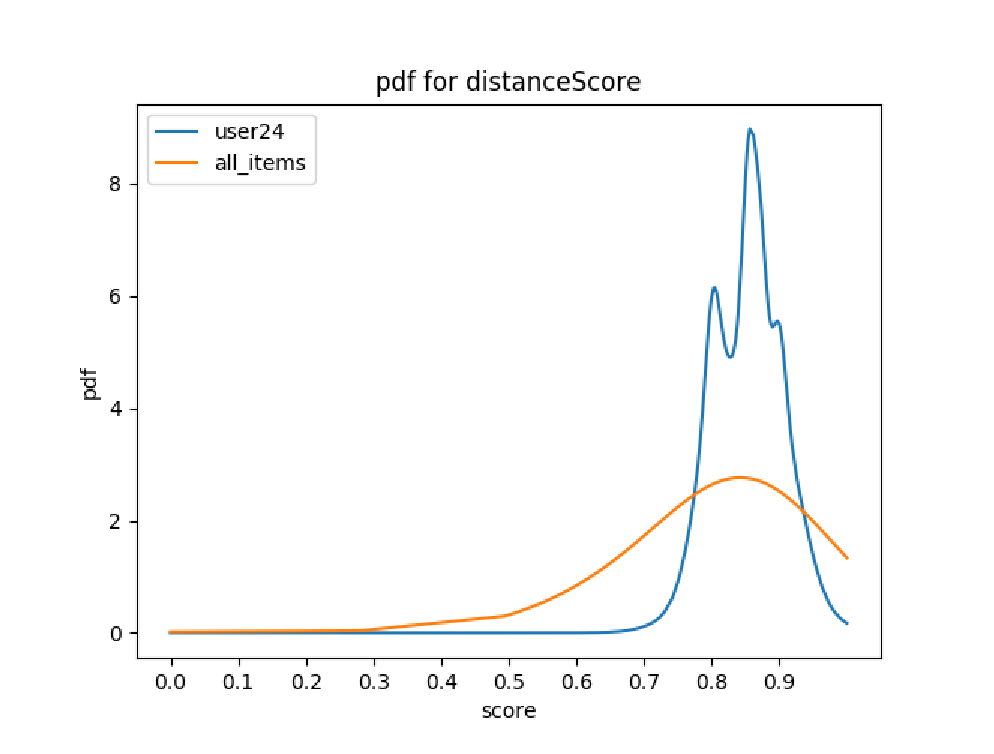
\includegraphics[width=6in]{source/ROLE7-distance.eps}
  \vspace{1mm}
  \caption{ROLE7の距離特徴量分布} %\vspace{-3mm}
  \label{fig:ROLE7-distance}
  %\vspace{-0.4cm}
  \end{center} 
\end{figure}

\begin{figure}[H]
  \begin{center}
    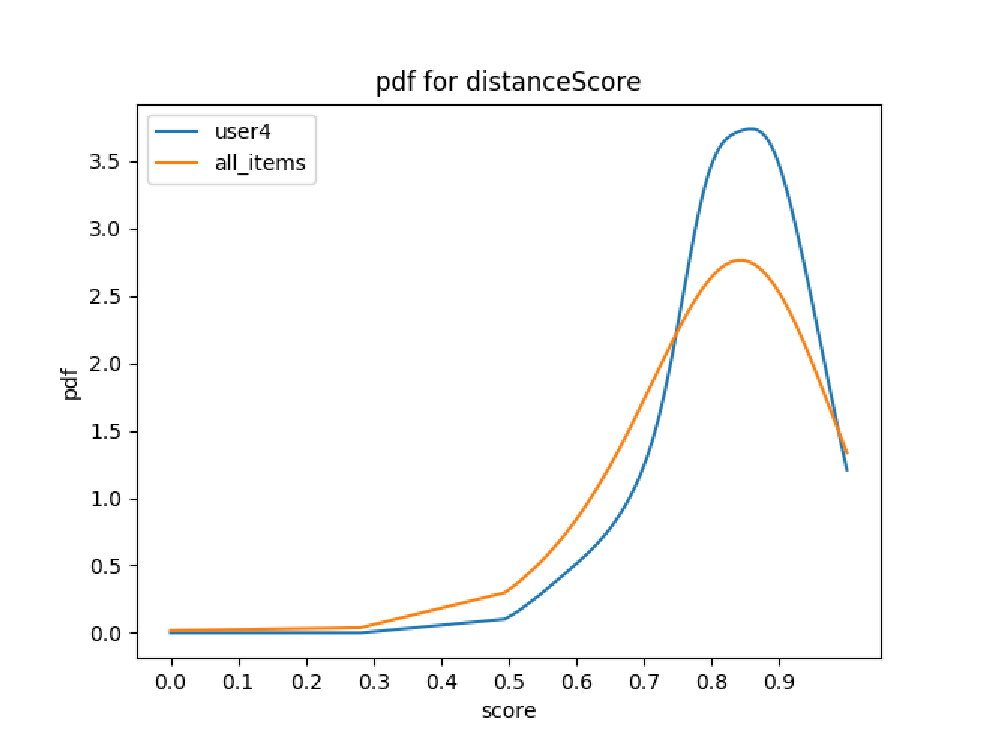
\includegraphics[width=6in]{source/ROLE1-distance.eps}
  \vspace{1mm}
  \caption{ROLE1の距離特徴量分布} %\vspace{-3mm}
  \label{fig:ROLE1-distance}
  %\vspace{-0.4cm}
  \end{center} 
\end{figure}

\begin{figure}[H]
  \begin{center}
    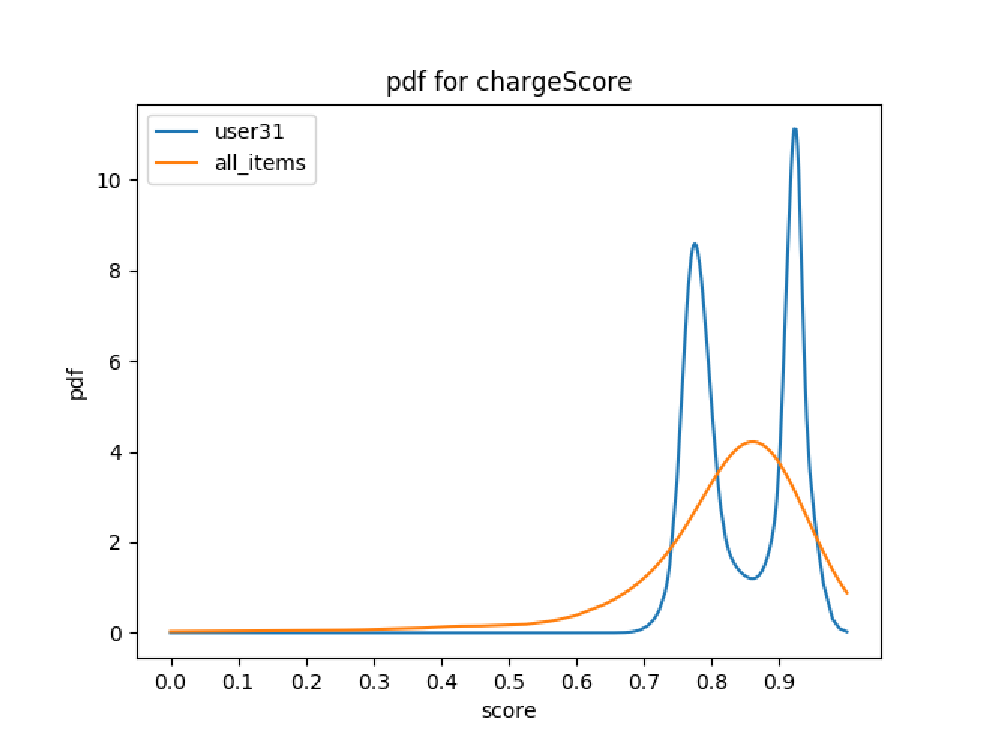
\includegraphics[width=6in]{source/ROLE14-charge.eps}
  \vspace{1mm}
  \caption{ROLE14の価格特徴量分布} %\vspace{-3mm}
  \label{fig:ROLE14-charge}
  %\vspace{-0.4cm}
  \end{center} 
\end{figure}



\begin{table*}[h]
  \caption{旧データセットでの実験結果} 
  \label{tbl:resultOld}
  \begin{center} {
\scalebox{0.9}[1]{
    \begin{tabular}{|l|l|l|ll|} \hline
      measure&$C_{Kd,Shr,Tl}$(提)&$C_{Nrm,Inf}$(既)&$LIN$&$SVM$\\ \hline
iP@0&1.0&0.995&0.98&0.991\\
iP@0.1&0.994&0.992&0.959&0.986\\
iP@0.2&0.976&0.99&0.94&0.981\\
iP@0.3&0.954&0.955&0.918&0.965\\
iP@0.4&0.92&0.934&0.884&0.958\\
iP@0.5&0.899&0.922&0.849&0.945\\
iP@0.6&0.848&0.888&0.811&0.913\\
iP@0.7&0.808&0.845&0.772&0.863\\
iP@0.8&0.755&0.756&0.709&0.814\\
iP@0.9&0.696&0.64&0.633&0.741\\
iP@1.0&0.568&0.503&0.531&0.634\\ \hline
MAiP&0.856&0.856&0.817&0.89\\ \hline
nDCG@5&0.995&0.992&0.96&0.981\\
nDCG@10&0.987&0.987&0.957&0.98\\
nDCG@15&0.981&0.981&0.952&0.977\\
nDCG@20&0.975&0.978&0.949&0.974\\
nDCG@30&0.967&0.972&0.942&0.969\\ \hline
P@5&0.954&0.954&0.887&0.946\\
P@10&0.888&0.9&0.862&0.923\\
P@15&0.81&0.847&0.799&0.857\\
P@20&0.764&0.775&0.732&0.794\\
P@30&0.648&0.638&0.617&0.669\\ \hline
\end{tabular}
  }
    }
  \end{center}
\end{table*}

\begin{table*}[h]
  \caption{旧データセットでの提案手法との比較におけるU検定でのp値} 
  \label{tbl:resultOldUP}
  \begin{center} {
\scalebox{0.9}[1]{
\begin{tabular}{|l|l|ll|} \hline
measure&$C_{Nrm,Inf}$(既)&$LIN$&$SVM$\\ \hline
iP@0&0.359&0.079&0.166\\
iP@0.1&0.965&0.013&0.383\\
iP@0.2&0.449&0.112&0.777\\
iP@0.3&0.952&0.13&0.953\\
iP@0.4&0.93&0.224&0.485\\
iP@0.5&0.644&0.175&0.401\\
iP@0.6&0.544&0.47&0.341\\
iP@0.7&0.488&0.583&0.47\\
iP@0.8&0.931&0.544&0.402\\
iP@0.9&0.47&0.624&0.402\\
iP@1.0&0.544&0.773&0.371\\ \hline
MAiP&0.977&0.402&0.436\\ \hline
nDCG@5&0.535&0.055&0.468\\
nDCG@10&0.839&0.093&0.643\\
nDCG@15&0.954&0.088&0.794\\
nDCG@20&0.664&0.106&1.0\\
nDCG@30&0.665&0.184&0.908\\ \hline
P@5&0.697&0.084&0.622\\
P@10&0.861&0.561&0.6\\
P@15&0.562&0.817&0.524\\
P@20&0.908&0.665&0.729\\
P@30&0.862&0.729&0.84\\ \hline
\end{tabular}
  }
    }
  \end{center}
\end{table*}

\begin{comment}
\begin{table*}[h]
  \caption{旧データセットでの提案手法との比較におけるt検定でのp値} 
  \label{tbl:resultOldTP}
  \begin{center} {
\scalebox{0.9}[1]{
\begin{tabular}{|l|l|ll|} \hline
$measure$&$C_{Nrm,Inf}$&$LIN$&$SVM$\\ \hline
iP@0&0.339&0.143&0.196\\
iP@0.1&0.787&0.047&0.38\\
iP@0.2&0.361&0.184&0.742\\
iP@0.3&0.966&0.257&0.614\\
iP@0.4&0.706&0.365&0.239\\
iP@0.5&0.568&0.259&0.187\\
iP@0.6&0.435&0.497&0.15\\
iP@0.7&0.551&0.572&0.302\\
iP@0.8&0.99&0.504&0.343\\
iP@0.9&0.459&0.374&0.498\\
iP@1.0&0.414&0.629&0.397\\ \hline
MAiP&1.0&0.336&0.319\\ \hline
nDCG@5&0.643&0.068&0.204\\
nDCG@10&0.913&0.061&0.401\\
nDCG@15&0.968&0.07&0.683\\
nDCG@20&0.749&0.11&0.981\\
nDCG@30&0.676&0.137&0.864\\ \hline
P@5&1.0&0.115&0.752\\
P@10&0.77&0.58&0.368\\
P@15&0.54&0.847&0.407\\
P@20&0.88&0.654&0.663\\
P@30&0.903&0.692&0.8\\ \hline
\end{tabular}
  }
    }
  \end{center}
\end{table*}
\end{comment}

\subsection{旧データセットでの実験結果}
実験結果は表\ref{tbl:resultOld}である.
鈴木らの既存手法は$C_{Nrm,Inf}$で,提案手法は$C_{Kd,Shr,Tl}$であることに注意する.
提案手法と各比較手法で平均差がない,という仮説におけるマンホイットニーのU検定ときのp値の結果が表\ref{tbl:resultOldUP}である.\par
表\ref{tbl:resultOldUP}から,全ての評価指標で既存手法と提案手法でp値が30\%以上であることがわかる\par
よって既存手法と提案手法に有意な差はないと判断できるため,旧データセットに対して提案手法は,既存手法と同等の性能を示すといえる.
\subsection{新データセットでの実験結果}
実験結果は表\ref{tbl:resultNew}である.\par
検索結果上位に対する評価指標を含めた過半数の評価指標で,提案手法が比較手法よりも優れた結果を示している.\par
提案手法と各比較手法で平均差がない,という帰無仮説におけるマンホイットニーのU検定をしたときのp値の結果が表\ref{tbl:resultNewP}である.
既存手法におけるp値は全評価指標において1\%未満である.
よって,提案手法は既存手法と比較して有意水準1\%以下で性能がよいといえる.\par
以下で指摘した問題ケースごとの結果について分析する.
\begin{itemize}
  \item {\bf 喫煙値について偏った嗜好をもつケース}\par
    結果は表\ref{tbl:resultSmoke}である.\par
提案手法が比較手法の過半数で,$SVM$に次いで,最高の結果を示しており,\ref{ch:proposal}章で提案した各小手法を部分的に組み合わせたどの手法よりも,優れた結果を示している.
    また,関心度式に$Att_{Shr}$を採用する手法が,$Att_{Inf}$を採用する手法よりも優れた結果を示す傾向が通常のケース(表\ref{tbl:resultNormal})より顕著である.\par
  よって離散値特徴量を扱う場合,$Att_{Shr}$が$Att_{Inf}$よりもより有効に機能するといえる.
  \item {\bf 特異な分布ケース}\par
    表\ref{tbl:ROLE}のROLE7やROLE14のような特異な嗜好ケースに対する結果は,表\ref{tbl:resultUshape}である.\par
    提案手法が比較手法の過半数で,最高の結果を示している.また,フィルターを有効にする手法が,フィルターを有効にしない手法より優れた結果を示す傾向が通常のケース(図\ref{tbl:resultNormal})よりも顕著である.\par
    よって,フィルターが有効に機能しているといえる.
\end{itemize}
\par

通常のケースだけでなく,離散値について偏った嗜好を持つケース(表\ref{tbl:resultSmoke})や,表\ref{tbl:ROLE}のROLE7やROLE14のような特異な嗜好ケース(表\ref{tbl:resultUshape})においても,提案手法は過半数の評価指標で最高の結果あるいは$SVM$に次ぐ結果を示すことから,提案手法は他の比較手法と比較して評価実験で用いたような複雑な嗜好ケースにおいても安定した結果を示す手法であることがわかる.

\begin{table*}[h]
 \caption{新データセットでの実験結果} 
\label{tbl:resultNew}
  \begin{center} {
\scalebox{0.9}[1]{
    \begin{tabular}{|l|l|l|lllll|}\hline
measure&$C_{Kd,Shr,Tl}$(提)&$C_{Nrm,Inf}$(既)&$C_{Kd,Inf,Tl}$&$C_{Kd,Shr}$&$C_{Kd,Inf}$&$LIN$&$SVM$\\ \hline
iP@0&0.98&0.706&0.963&0.937&0.908&0.87&0.953\\
iP@0.1&0.968&0.63&0.939&0.901&0.871&0.862&0.941\\
iP@0.2&0.955&0.575&0.903&0.867&0.838&0.84&0.927\\
iP@0.3&0.931&0.539&0.876&0.842&0.808&0.803&0.9\\
iP@0.4&0.911&0.513&0.852&0.825&0.792&0.787&0.871\\
iP@0.5&0.875&0.502&0.802&0.804&0.769&0.753&0.844\\
iP@0.6&0.838&0.482&0.745&0.769&0.736&0.711&0.806\\
iP@0.7&0.797&0.467&0.698&0.738&0.696&0.675&0.769\\
iP@0.8&0.731&0.454&0.639&0.691&0.647&0.635&0.731\\
iP@0.9&0.653&0.43&0.586&0.624&0.599&0.594&0.663\\
iP@1.0&0.55&0.405&0.515&0.55&0.518&0.527&0.581\\ \hline
MAiP&0.835&0.518&0.774&0.777&0.744&0.733&0.817\\ \hline
nDCG@5&0.963&0.681&0.948&0.892&0.877&0.779&0.941\\
nDCG@10&0.96&0.702&0.938&0.901&0.875&0.814&0.939\\
nDCG@15&0.954&0.715&0.932&0.899&0.879&0.832&0.937\\
nDCG@20&0.951&0.718&0.927&0.899&0.88&0.84&0.934\\
nDCG@30&0.945&0.728&0.918&0.898&0.879&0.852&0.928\\ \hline
P@5&0.891&0.455&0.847&0.77&0.755&0.682&0.865\\
P@10&0.843&0.467&0.768&0.746&0.716&0.671&0.812\\
P@15&0.781&0.443&0.712&0.703&0.682&0.64&0.762\\
P@20&0.711&0.445&0.65&0.667&0.634&0.604&0.714\\
P@30&0.597&0.432&0.562&0.586&0.564&0.541&0.614\\ \hline
    \end{tabular}
  }
    }
  \end{center}
\end{table*}

\begin{table*}[h]
  \caption{新データセットでの提案手法との比較におけるU検定でのp値}
\label{tbl:resultNewP}
  \begin{center} {
\scalebox{0.9}[1]{
    \begin{tabular}{|l|l|lllll|}\hline
measur&$C_{Nrm,Inf}$(既)&$C_{Kd,Inf,Tl}$&$C_{Kd,Shr}$&$C_{Kd,Inf}$&$LIN$&$SVM$\\ \hline
iP@0&0.0&0.251&0.064&0.011&0.0&0.458\\
iP@0.1&0.0&0.324&0.125&0.02&0.005&0.707\\
iP@0.2&0.0&0.035&0.036&0.017&0.003&0.631\\
iP@0.3&0.0&0.041&0.047&0.01&0.001&0.37\\
iP@0.4&0.0&0.027&0.055&0.006&0.0&0.089\\
iP@0.5&0.0&0.036&0.139&0.024&0.003&0.234\\
iP@0.6&0.0&0.021&0.161&0.036&0.008&0.215\\
iP@0.7&0.0&0.015&0.18&0.035&0.018&0.306\\
iP@0.8&0.0&0.04&0.308&0.084&0.059&0.564\\
iP@0.9&0.0&0.064&0.313&0.119&0.144&0.682\\
iP@1.0&0.001&0.21&0.513&0.263&0.338&0.8\\ \hline
MAiP&0.0&0.043&0.197&0.029&0.017&0.561\\ \hline
nDCG@5&0.0&0.231&0.048&0.014&0.001&0.497\\
nDCG@10&0.0&0.174&0.086&0.023&0.001&0.482\\
nDCG@15&0.0&0.125&0.093&0.024&0.001&0.487\\
nDCG@20&0.0&0.089&0.095&0.021&0.002&0.396\\
nDCG@30&0.0&0.066&0.115&0.019&0.003&0.409\\ \hline
P@5&0.0&0.178&0.073&0.04&0.003&0.484\\
P@10&0.0&0.05&0.084&0.022&0.004&0.369\\
P@15&0.0&0.125&0.117&0.052&0.01&0.439\\
P@20&0.0&0.151&0.271&0.135&0.051&0.579\\
P@30&0.003&0.246&0.424&0.261&0.168&0.633\\ \hline
    \end{tabular}
  }
    }
  \end{center}
\end{table*}


\begin{table*}[h]
  \caption{新データセットにおける通常の分布の実験結果} 
  \label{tbl:resultNormal}
  \begin{center} {
\scalebox{0.9}[1]{
    \begin{tabular}{|l|l|l|lllll|}\hline
measure&$C_{Kd,Shr,Tl}$(提)&$C_{Nrm,Inf}$(既)&$C_{Kd,Inf,Tl}$&$C_{Kd,Shr}$&$C_{Kd,Inf}$&$LIN$&$SVM$\\ \hline
iP@0&0.973&0.705&0.962&0.918&0.903&0.836&0.936\\
iP@0.1&0.958&0.632&0.942&0.873&0.86&0.83&0.921\\
iP@0.2&0.947&0.578&0.905&0.833&0.823&0.806&0.902\\
iP@0.3&0.919&0.535&0.881&0.802&0.791&0.761&0.869\\
iP@0.4&0.895&0.511&0.864&0.784&0.774&0.74&0.839\\
iP@0.5&0.856&0.499&0.833&0.758&0.754&0.701&0.808\\
iP@0.6&0.818&0.477&0.776&0.719&0.72&0.652&0.771\\
iP@0.7&0.785&0.462&0.729&0.691&0.68&0.619&0.733\\
iP@0.8&0.719&0.448&0.663&0.645&0.637&0.583&0.691\\
iP@0.9&0.657&0.425&0.61&0.594&0.596&0.555&0.618\\
iP@1.0&0.559&0.412&0.54&0.535&0.532&0.509&0.544\\ \hline
MAiP&0.826&0.517&0.791&0.741&0.734&0.69&0.785\\ \hline
nDCG@5&0.953&0.684&0.947&0.863&0.864&0.733&0.92\\
nDCG@10&0.951&0.702&0.937&0.877&0.862&0.776&0.919\\
nDCG@15&0.944&0.717&0.934&0.875&0.868&0.798&0.919\\
nDCG@20&0.941&0.718&0.928&0.875&0.87&0.807&0.916\\
nDCG@30&0.935&0.727&0.921&0.874&0.869&0.821&0.911\\ \hline
P@5&0.869&0.46&0.85&0.712&0.725&0.627&0.829\\
P@10&0.819&0.472&0.784&0.697&0.699&0.611&0.779\\
P@15&0.758&0.447&0.728&0.654&0.672&0.584&0.726\\
P@20&0.697&0.449&0.673&0.627&0.628&0.555&0.683\\
P@30&0.609&0.441&0.584&0.573&0.567&0.514&0.601\\ \hline
\end{tabular}
  }
    }
  \end{center}
\end{table*}

\begin{table*}[h]
  \caption{喫煙値を重視したユーザ集合での実験結果} 
  \label{tbl:resultSmoke}
  \begin{center} {
\scalebox{0.9}[1]{
    \begin{tabular}{|l|l|l|lllll|}\hline
measure&$C_{Kd,Shr,Tl}$(提)&$C_{Nrm,Inf}$(既)&$C_{Kd,Inf,Tl}$&$C_{Kd,Shr}$&$C_{Kd,Inf}$&$LIN$&$SVM$\\ \hline
iP@0&0.997&0.709&0.966&0.986&0.922&0.96&1.0\\
iP@0.1&0.994&0.624&0.93&0.976&0.899&0.948&0.993\\
iP@0.2&0.977&0.567&0.898&0.956&0.88&0.933&0.992\\
iP@0.3&0.962&0.548&0.863&0.95&0.855&0.917&0.982\\
iP@0.4&0.952&0.517&0.821&0.936&0.841&0.91&0.958\\
iP@0.5&0.926&0.508&0.718&0.924&0.811&0.892&0.937\\
iP@0.6&0.892&0.495&0.661&0.902&0.78&0.869&0.899\\
iP@0.7&0.83&0.48&0.614&0.863&0.738&0.825&0.867\\
iP@0.8&0.762&0.469&0.576&0.815&0.673&0.773&0.838\\
iP@0.9&0.641&0.442&0.52&0.704&0.607&0.699&0.781\\
iP@1.0&0.525&0.386&0.448&0.59&0.478&0.575&0.68\\ \hline
MAiP&0.86&0.522&0.729&0.873&0.771&0.846&0.902\\ \hline
nDCG@5&0.989&0.675&0.949&0.969&0.911&0.899&0.996\\
nDCG@10&0.985&0.7&0.94&0.967&0.91&0.917&0.989\\
nDCG@15&0.981&0.711&0.929&0.965&0.908&0.925&0.984\\
nDCG@20&0.978&0.718&0.925&0.964&0.908&0.93&0.98\\
nDCG@30&0.971&0.729&0.911&0.96&0.907&0.933&0.974\\ \hline
P@5&0.95&0.439&0.839&0.922&0.833&0.828&0.961\\
P@10&0.908&0.456&0.725&0.878&0.761&0.831&0.9\\
P@15&0.843&0.431&0.669&0.831&0.707&0.791&0.859\\
P@20&0.749&0.435&0.588&0.774&0.65&0.736&0.799\\
P@30&0.568&0.407&0.502&0.621&0.556&0.613&0.648\\ \hline
\end{tabular}
  }
    }
  \end{center}
\end{table*}

\begin{table*}[h]
  \caption{特異な分布での実験結果} 
  \label{tbl:resultUshape}
  \begin{center} {
\scalebox{0.9}[1]{
    \begin{tabular}{|l|l|l|lllll|}\hline
measure&$C_{Kd,Shr,Tl}$(提)&$C_{Nrm,Inf}$(既)&$C_{Kd,Inf,Tl}$&$C_{Kd,Shr}$&$C_{Kd,Inf}$&$LIN$&$SVM$\\ \hline
iP@0&0.958&0.65&0.94&0.869&0.847&0.745&0.898\\
iP@0.1&0.942&0.588&0.914&0.804&0.783&0.741&0.875\\
iP@0.2&0.924&0.511&0.857&0.741&0.723&0.708&0.854\\
iP@0.3&0.884&0.454&0.821&0.694&0.676&0.646&0.807\\
iP@0.4&0.85&0.423&0.802&0.671&0.654&0.624&0.768\\
iP@0.5&0.804&0.407&0.76&0.638&0.629&0.572&0.727\\
iP@0.6&0.753&0.384&0.682&0.587&0.585&0.512&0.679\\
iP@0.7&0.716&0.368&0.627&0.555&0.538&0.481&0.634\\
iP@0.8&0.631&0.357&0.548&0.504&0.492&0.445&0.579\\
iP@0.9&0.561&0.335&0.483&0.454&0.458&0.42&0.495\\
iP@1.0&0.461&0.324&0.433&0.429&0.431&0.391&0.441\\ \hline
MAiP&0.771&0.437&0.715&0.632&0.62&0.571&0.705\\ \hline
nDCG@5&0.934&0.618&0.922&0.789&0.79&0.589&0.877\\
nDCG@10&0.93&0.638&0.907&0.81&0.786&0.656&0.878\\
nDCG@15&0.92&0.659&0.902&0.807&0.795&0.692&0.879\\
nDCG@20&0.915&0.661&0.894&0.808&0.799&0.708&0.875\\
nDCG@30&0.907&0.671&0.884&0.809&0.799&0.733&0.868\\ \hline
P@5&0.813&0.37&0.777&0.56&0.573&0.437&0.747\\
P@10&0.742&0.363&0.687&0.542&0.547&0.43&0.682\\
P@15&0.669&0.344&0.619&0.502&0.523&0.413&0.62\\
P@20&0.598&0.352&0.558&0.481&0.482&0.402&0.573\\
P@30&0.505&0.341&0.467&0.441&0.433&0.373&0.482\\ \hline
\end{tabular}
  }
    }
  \end{center}
\end{table*}
\clearpage
\begin{comment}
\begin{table*}[h]
  \caption{喫煙値を重視したユーザ集合での実験結果} 
  \label{tbl:resultSmoke}
  \begin{center} {
\scalebox{0.9}[1]{
    \begin{tabular}{|l|l|l|l|l|} \hline
      measure&$C_{Kd,Shr,Tl}$(提)&$C_{Nrm,Inf}$(既)&$LIN$&$SVM$\\ \hline
\end{tabular}
  }
    }
  \end{center}
\end{table*}
\end{comment}
